\documentclass[11pt]{article}

% ==== Paquetes ====
\usepackage[utf8]{inputenc}
\usepackage[spanish]{babel}
\usepackage{amsmath, amssymb, amsfonts, siunitx}
\usepackage{graphicx}
\usepackage{float}
\usepackage{minted}   % Para código con sintaxis coloreada
\usepackage{xcolor}
\usepackage{hyperref}
\usepackage{caption}
\usepackage{subcaption}
\usepackage{geometry}
\usepackage{listings}
\usepackage{tikz}

\lstset{basicstyle=\ttfamily\small,breaklines=true}

\geometry{margin=2.5cm}

% ==== Datos de la tarea ====
\title{IEE3584 - Comunicaciones inalámbricas \\
Tarea 5}
\author{Nicolás Seguel}
\date{Septiembre 2025}

\begin{document}
\maketitle

\section*{Problema 9:}

El presupuesto de enlace para \(\SI{1.8}{GHz}\) es la siguiente:
\begin{center}
    \begin{tabular}{|c|c|c|}
        \hline
        \(P_t\) & dBW & \(-10\) \\
        \(\delta_t\) & dB & \(+4.8 \cdot 3\) \\
        \(\Lambda_p\) & dB & \(-136.92\) \\
        \(\delta_r\) & dB & \(+0\) \\
        \(\omega_t\) & dB & \(-151\) \\
        \(\omega_{fig}\) & dB & \(7.6\) \\
        \(outage\) & dB & \(10\) \\
        \(SNR\) & dB & \(7.5\) \\
        \hline
    \end{tabular}
\end{center}

Se tiene que la potencia transmitida es \(\SI{100}{mW}\) o \(\SI{-10}{dBW}\), la ganacia de la antena transmisora es \(\SI{4.8}{dB}\) y se recibe de tres antenas, la perdida por distancia para \(\SI{360}{m}\) con una distancia de referencia de \(\SI{10}{m}\) para \(\SI{1.8}{GHz}\) es \(\SI{-136.92}{dB}\). Luego, la ganacia de la antena receptora es \(\SI{0}{dB}\), el ruido térmico para un ancho de banda de \(\SI{200}{kHz}\) (segun Wikipedia) es \(\SI{-151}{dB}\), la figura de ruido es \(\SI{7.6}{dB}\), el margen de cobertura \(\SI{-10}{dB}\), según la tabla vista en clases y se quiere una SNR de \(\SI{7.5}{dB}\).

\begin{equation}
    P_t + 14.4 - 136.92 + 0 + 151 - 7.6 - 10 \geq 7.5
\end{equation}

\begin{equation}
    -10 \geq \SI{-3.38}{dBW}
\end{equation}

Para \(\SI{900}{MHz}\), lo único que cambia es la pérdida de potencia por distancia, que es igual a \(\SI{-130.90}{dB}\).

\begin{equation}
    P_t + 14.4 - 130.90 + 0 + 151 - 7.6 - 10 \geq 7.5
\end{equation}

\begin{equation}
    -10 \geq \SI{-9.4}{dBW}
\end{equation}

El presupuesto de enlace calculado es válido para los \(\SI{900}{MHz}\).

\section*{Problema 10:}

\subsection*{Presupuesto de enlace}

La potencia de la antena transmisora tiene que ser de al menos \(\SI{-3.38}{dBW}\), como se calculó en el inciso anterior.

\subsection*{Radio para una potencia de \(\SI{100}{mW}\)}

Para que se cumpla el presupuesto de enlace la pérdida de potencia por distancia tiene que ser \(\SI{6.6}{dB}\) mayor que para el caso anterior, por lo que despejando se tiene que:

\begin{equation*}
    d = 10^{\frac{79.37- 6.6}{51}+1}
\end{equation*}

La distancia para que se cumpla el nuevo presupuesto de enlace es \(d = \SI{267.23}{m}\).

\subsection*{Probabilidad de cobertura}

Se tiene que la probabilidad de cobertura es:

\begin{equation*}
    1-P_{outage} = e^{-\Gamma_{min}/\bar{\gamma}}
\end{equation*}

Con \(\Gamma_{min} = \SI{5.62}{}\) y \(\bar{\gamma} = \SI{12.24}{}\), despejando del presupuesto de enlace de la pregunta anterior, por lo que la probabilidad de cobertura es:

\begin{equation*}
    1-P_{outage} = 0.63
\end{equation*}

\section*{Problema 12:}

\begin{figure}[H]
    \centering
    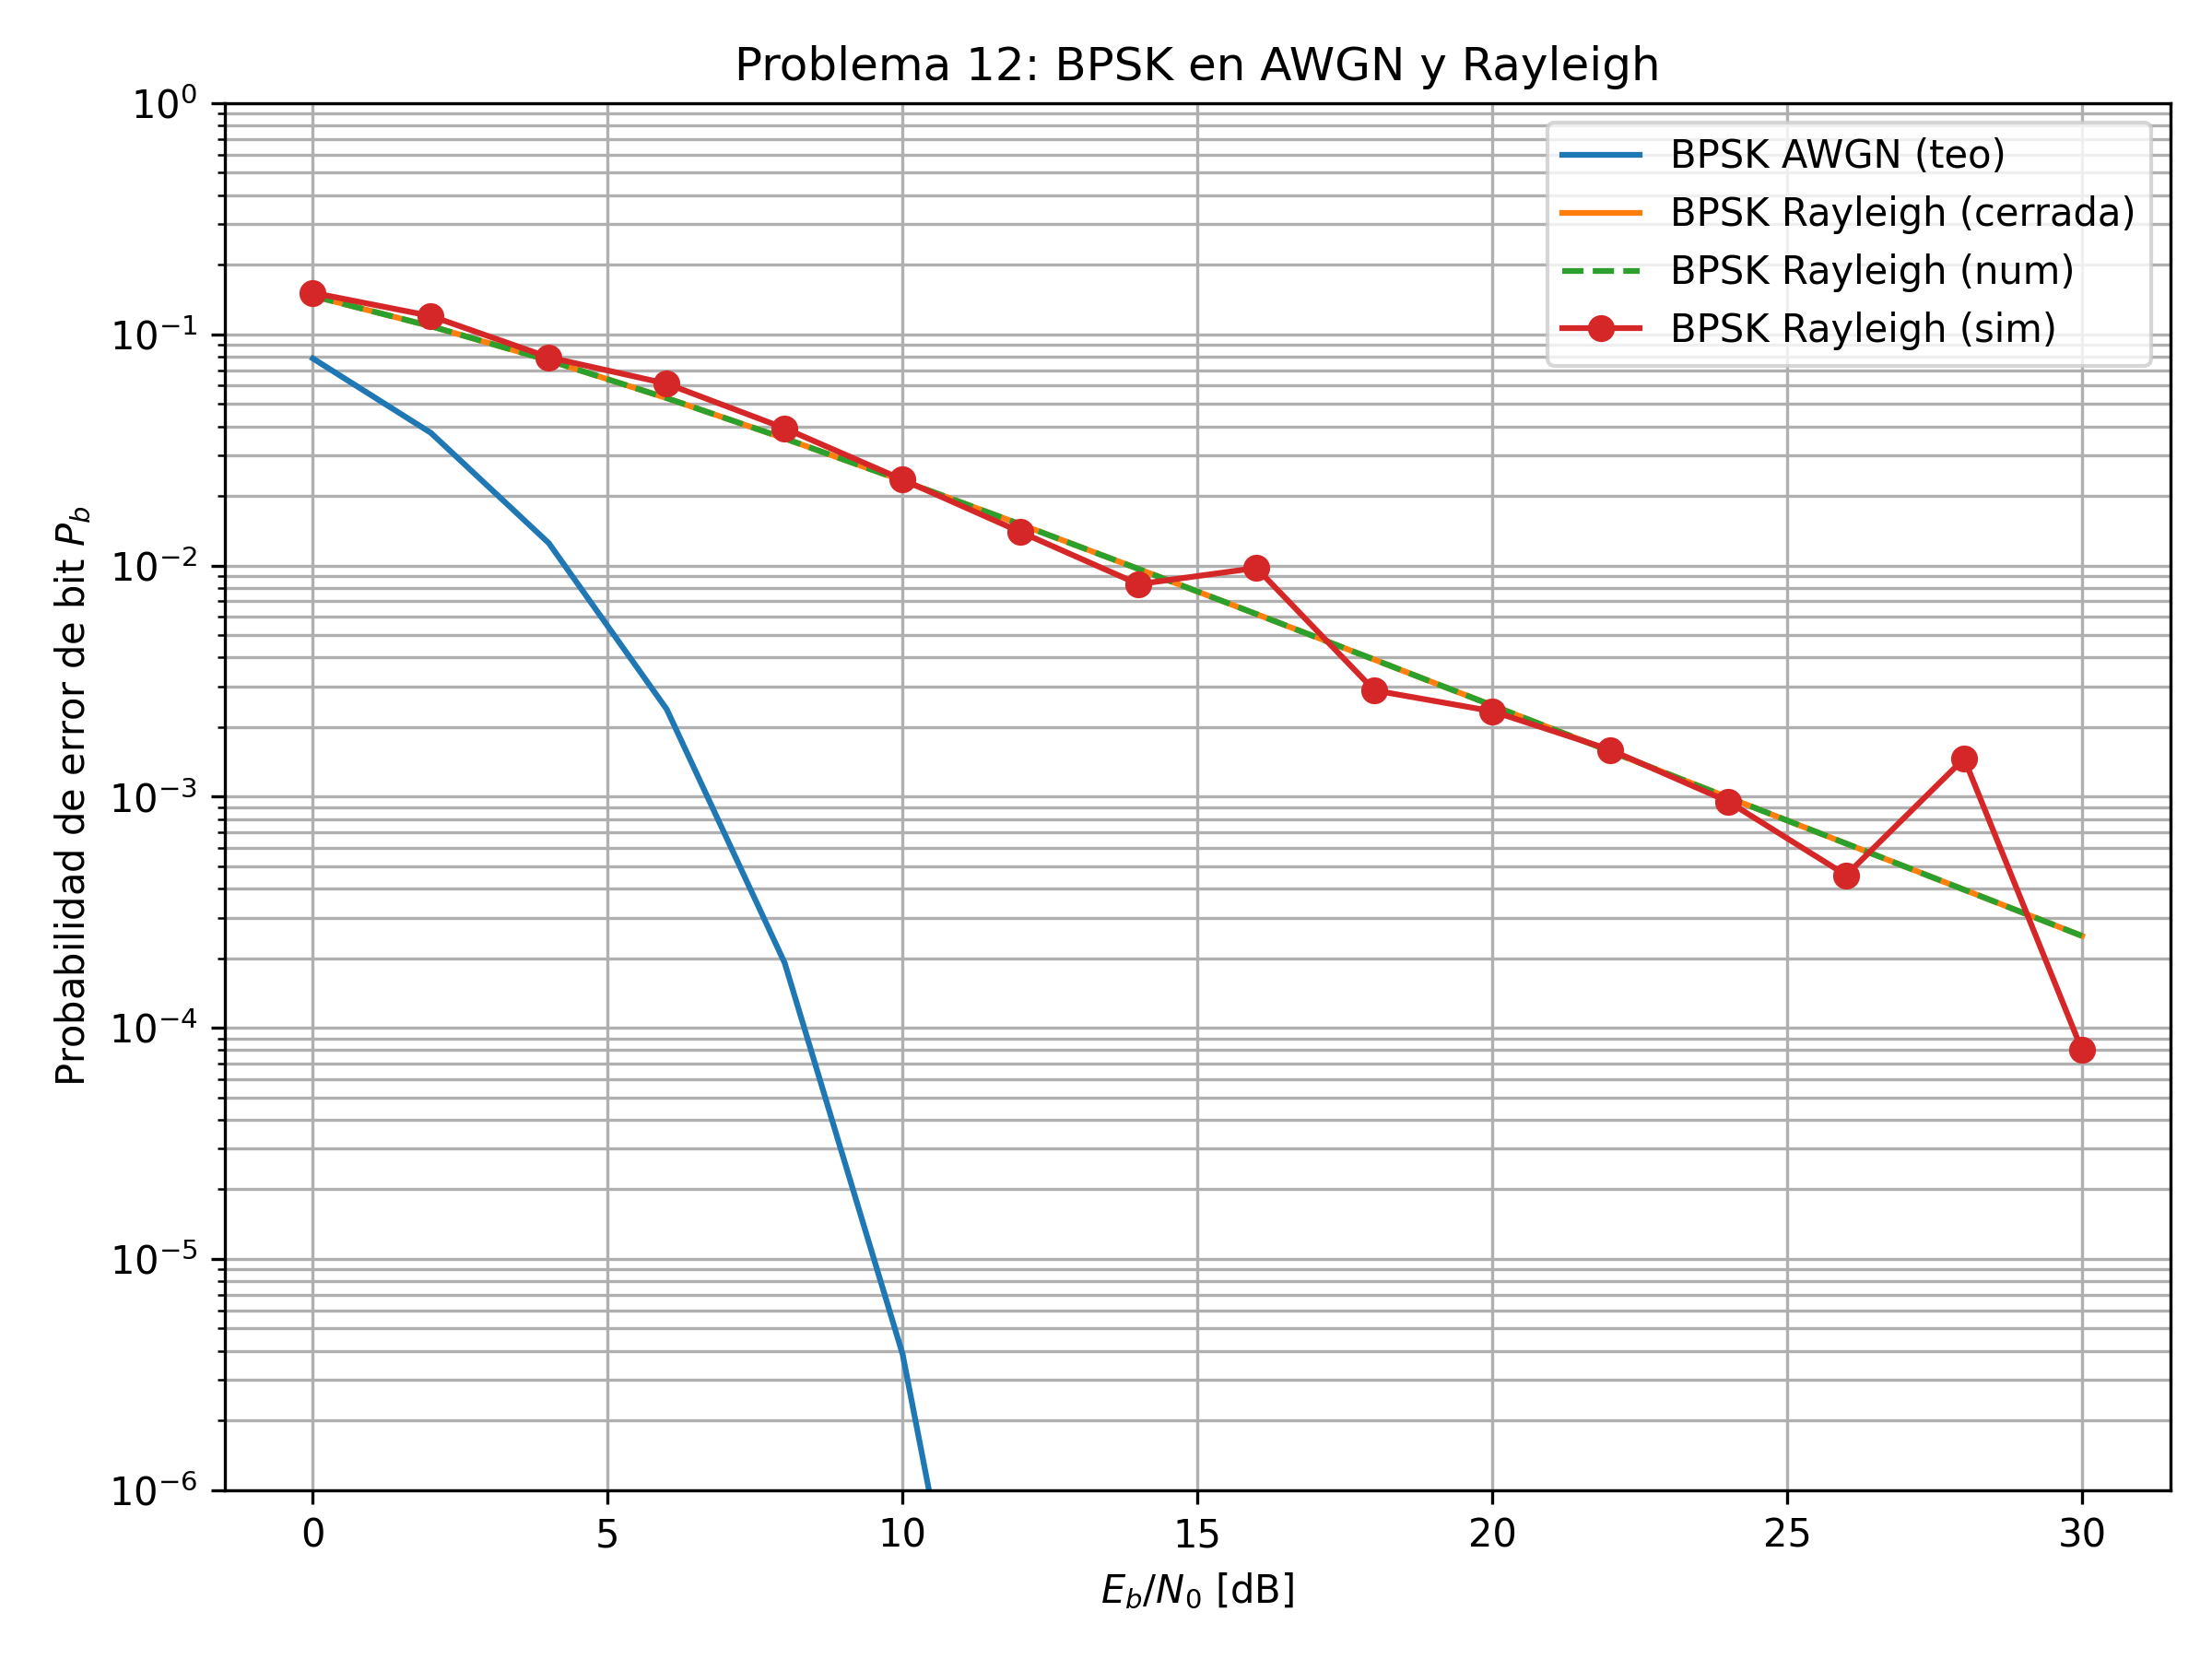
\includegraphics[width= 0.8\textwidth]{problema12_fig.png}
    \caption{}
\end{figure}

Se utilizó asistencia de una IA para hacer los calculos en la parte \textbf{d} del gráfico.

\lstinputlisting[language=Python]{problema12.py}

\section*{Problema 13:}

La probabilidad de error media se obtiene promediando sobre todos los modos y sobre la
distribución de $\gamma$:

\begin{equation}
    \overline{P_b} = \sum_{i=1}^{N} \int_{\Gamma_i}^{\Gamma_{i+1}}
    P_b^{(i)}(\gamma)\, p_\gamma(\gamma)\, d\gamma,
\end{equation}

donde $p_\gamma(\gamma) = \dfrac{1}{\bar{\gamma}} e^{-\gamma/\bar{\gamma}}$ para desvanecimiento Rayleigh.

(se me acabo el tiempo, esto es todo lo que pude hacer)

\end{document}
